\chapter{Nghiên cứu hệ thống chỉ đường}
\label{Chapter3}

\emph{Chương này sẽ trình bày, mô tả chi tiết về các nghiên cứu đã được thực hiện để giải quyết bài toán chỉ đường, bao gồm danh sách và việc lựa chọn một số thuật toán xử lí giọng nói
}

Sơ đồ của hệ thống chỉ đường: 


Khi người dùng gửi một câu truy vấn bằng audio thì sẽ chuyển giọng nói đó thành văn bản (speech to text) 
văn bản đó được gửi tới NLU engine để trích xuất ý định và các thực thể 
Dựa trên ý định và thực thể nhận được sẽ tạo ra câu trả lời tương ứng và trả về cho người dùng bằng text và audio ( text to speech để chuyển văn bản thành giọng nói) 

Các dữ liệu về đường đi được truy vấn từ google map API. 
speech to text và text to speech sử dụng thư viện có sẵn
nghiên cứu sử dụng công cụ có sẵn Snips NLU cho việc trích xuất ý định và các thực thể 

Snips NLU là công cụ giúp hiểu ngôn ngữ tự nhiên mạnh mẽ, nhưng hiện tại chưa hỗ trợ tiếng Việt, ý tưởng của nhóm em là sẽ tạo một bộ dữ liệu bằng tiếng Việt rồi dịch sang tiếng Anh, dùng dữ liệu tiếng Anh đó để huấn luyện cho mô hình. Khi người dùng truy vấn thì dịch câu truy vấn đó sang tiếng Anh và đưa vào mô hình để trích xuất ý định và các thực thể. 

Về mặt dữ liệu:
Định dạng bộ dữ liệu huấn luyện là ở dạng json 
Nhóm e có viết 1 chương trình nhỏ để hỗ trợ tạo dữ liệu
Dữ liệu gồm 2 intent là findRoute và askLocation. Mỗi intent gồm 20 câu huấn luyện và 10 câu để kiểm thử 
\section{Dịch}
Đầu tiên nhóm em dịch bộ dữ liệu bằng cách tách 1 câu thành từng từ rồi sử dụng thư viện (word2word) để dịch sang tiếng Anh.
Sau khi dịch ta được bộ dữ liệu như sau:
https://drive.google.com/file/d/1yoQk3AuViJpkcDQumQI-SbIw_iGyaGoJ/view?usp=sharing
https://drive.google.com/file/d/1i2YNlvZTVsTU2WrzIMBmxl4FcJuAtVyV/view?usp=sharing
Kết quả thu được: 
https://drive.google.com/file/d/1e2Z0g4irQXqeNMzz4rP1UPQ3OKqYsMPI/view?usp=sharing

Nhận xét kết quả đạt được: 

Dịch word by word sẽ àm mất ý nghĩa của câu nói: 

đường đi từ công an Rạch Chiếc tới Nhà văn hóa thanh niên thành phố => đường gone từ peacock Homeland Rạch Chiếc tới Nhà essay hóa bars lustrums thành phố

các slot cần được trích xuất đã bị dịch ra và không còn ý nghĩa nữa, không thể dùng để tìm kiếm địa điểm này trên google map được.

để xử lý vấn đề này, nhóm em sẽ sử dụng thư viện để tách từ (word segmentation) và gán nhãn từ loại (pos tagging)

Trong tiếng Việt, dấu cách (space) không được sử dụng như 1 kí hiệu phân tách từ, nó chỉ có ý nghĩa phân tách các âm tiết với nhau. Do đó việc tách từ sẽ giúp cho việc dịch được chính xác hơn

để xử lý vấn đề những slot bị dịch thành tiếng Anh làm cho nó không còn ý nghĩa nữa, nhóm em nhận thấy rằng những slot này chủ yếu là danh từ, nên nhóm sẽ sử dụng pos tagging để gán nhãn từ loại, những từ nào thuộc danh từ thì sẽ không cho dịch thành tiếng Anh.

Sau khi áp dụng word segmentation và pos tagging lên bộ dữ liệu và sử dụng thư viện word2word để dịch thì đạt được bộ dữ liệu như sau:
https://drive.google.com/file/d/1riZLV1dam9U6q5fuutBFZkzpC6IGgvbb/view?usp=sharing
https://drive.google.com/file/d/1Jq1x3-owrcL1TN1igPr7HFNRxTk2emW2/view?usp=sharing

Sau khi huấn luyện mô hình và đem đi đánh giá nhóm nhận được kết quả như sau:
https://drive.google.com/file/d/1UU7_04Ps6WHZXSujZxNqaZKZhtvYsnrL/view?usp=sharing

Nhận xét kết quả đạt được: 
Đã xử lý được vấn đề dịch những slot làm mất ý nghĩa của chúng:
	đường đi từ công an Rạch Chiếc tới Nhà văn hóa thanh niên thành phố  =>
	đường gone từ công_an Rạch Chiếc tới Nhà văn hóa thanh_niên thành phố
	
độ chính xác về nhận diện ý định và thực thể cao (nhận diện intent f1-score = 0.9736842105263158 và slot = 0.85)

tuy nhiên vẫn còn gặp nhiều vấn đề về việc dịch: 
VD: [[('kí', 'N'), ('túc', 'V'), ('xá', 'V'), ('cỏ', 'N'), ('may', 'A')]]
 => kí túc xá cỏ Unfortunately
 
thực tế cả cụm từ "kí túc xá" là danh từ và cần được giữ nguyên, nhưng do bộ tách từ còn chưa chính xác dẫn đến việc dịch không hiệu quả.


để xử lý vấn đề này, nhóm sẽ xây dựng một bộ từ điển, bộ từ điển này nằm trong phạm vi hỏi đường nên có thể xây dựng được, từ đó việc dịch sẽ đạt hiệu quả hơn.

Để cải thiện quá trình dịch từ tiếng Việt sang tiếng Anh, nhóm chúng em đã quyết định xây dựng bộ từ điển riêng để có thể dịch được kết quả chính xác hơn.
Trong phạm vi các câu hỏi về đường đi, chúng em đã lựa chọn dịch khoảng 50 từ và các cụm từ. Các bước để dịch được dữ liệu như sau:
\begin{itemize}
    \item[--] Bước 1: Xây dựng bộ từ điển riêng biệt về chủ đề hỏi đường đi và chuyển hoá từ ngôn ngữ tiếng Việt sang tiếng Anh.
    \item[--] Bước 2: Tìm từ dài nhất trong câu có trong bộ từ điển.
    \item[--] Bước 3: Lấy nghĩa của từ tương ứng trong từ điển.
\end{itemize}
Trong quá trình nghiên cứu, chúng em nhận thấy bước 2 là bước thật sự cần thiết để có thể tìm được từ thích hợp nhất với bộ từ điển để có kết quả tốt nhất. Dưới đây là mô tả quá trình tìm từ dài nhất có trong từ điển mà nhóm chúng em thực hiện (Xem hình Tìm từ dài nhất \ref{fig:longest-word}).
    
\end{figure}.
\begin{itemize}
    \item[--] Input: "Đường đi từ Đại học Nông Lâm đến Ngã tư Thủ Đức""
    \item[--] Output: ["Đường đi", "từ", "Đại học Nông Lâm", "đến", "Ngã tư Thủ Đức"]
\end{itemize}
\begin{figure}[htp]
    \centering
    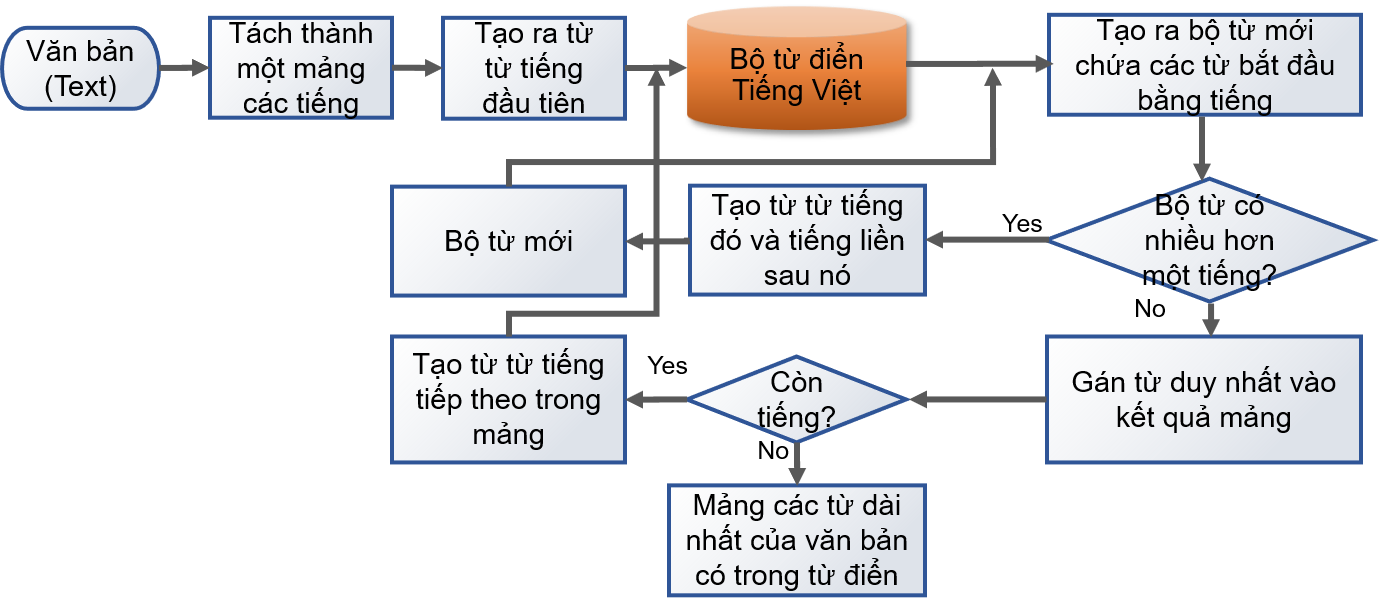
\includegraphics[width=10cm]{images/Diagram-longest-word.png}
    \caption{Tìm từ dài nhất}
    \label{fig:longest-word}
\end{figure}

